\documentclass[sigconf]{acmart}

\usepackage{graphicx}
\usepackage{algorithm} % for algorithms
\usepackage{algpseudocode}
\usepackage{booktabs} % For formal tables
\usepackage{amsthm} % For claims

\theoremstyle{remark}

\settopmatter{printacmref=false, printccs=true, printfolios=true}
\pagestyle{empty} % removes running headers

\newcommand{\PicScale}{0.5}
\newcommand {\FlameStream} {FlameStream}
\begin{document}

% \copyrightyear{2018} 
% \acmYear{2018} 
% \setcopyright{acmcopyright}
% \acmConference[BeyondMR'18]{Algorithms and Systems for MapReduce and Beyond }{June 15, 2018}{Houston, TX, USA}
% \acmBooktitle{BeyondMR'18: Algorithms and Systems for MapReduce and Beyond , June 15, 2018, Houston, TX, USA}
% \acmPrice{15.00}
% \acmDOI{10.1145/3206333.3209273}
% \acmISBN{978-1-4503-5703-6/18/06}

\title {Poster: decentralized validation of statistical properties in distributed stream processing}

\author{  Igor E. Kuralenok,$^1$     Artem Trofimov,$^ {1,2}$    Artem Permiakov,$^ {2}$   Andrey Pirozhkov,$^ {2}$    Semen Kutuzov,$^ {2}$     Arthur Nagaev,$^ {2}$    and  Boris Novikov$^ {1,2}$ }
\affiliation{%
\institution{$^1$JetBrains Research}
}
\affiliation{%
\institution{$^2$Saint Petersburg State University}
  \city{St. Petersburg} 
  \country{Russia}
}
\email{\string{ikuralenok, trofimov9artem\string}@gmail.com, borisnov@acm.org}

\begin{abstract}
State-of-the-art distributed stream processing systems are powerful tools for building latency-conscious scalable computational pipelines. With the complexity growth of these pipelines, the validation of the result has become a crucial task. In particular, testing that streaming data satisfies given statistical properties is an essential part of many real-life applications including machine learning, A/B testing, short-term personalization, etc. In this work, we highlight the problem of the applicability of such testing to streaming data that is partitioned among multiple computational units. We discuss the main challenges, possible solutions, and preliminary results.
\end{abstract}

% \keywords{Data streams, exactly-once, drifting state, optimistic OOP}

\maketitle

\thispagestyle{empty}

\section {Introduction}
\label {fs-short-intro}

%Refs:~\cite{Akidau:2013:MFS:2536222.2536229, Carbone:2017:SMA:3137765.3137777, Li2011, Li:2008:OPN:1453856.1453890, Murray:2013:NTD:2517349.2522738, Stonebraker:2005:RRS%:1107499.1107504, Zaharia:2012:DSE:2342763.2342773, we2018seim}

Exactly-once semantics even in a presence of failures is a desired property for stream processing systems~\cite{Akidau:2013:MFS:2536222.2536229}. One way to achieve it is to snapshot operations states atomically with respect to producing output~\cite{Carbone:2017:SMA:3137765.3137777} and to restart processing from the last successful snapshot on recovery. However, in this case, latency is up to the period of snapshotting. Another attractive approach is to make system idempotent, i.e., to ensure that input replay does not lead to duplicates on output. Google's MillWheel achieves idempotence by persistently logging each input item~\cite{Akidau:2013:MFS:2536222.2536229} and filtering out duplicates on recovery. This technique called {\em strong productions} limits the throughput of the operations by the throughput of logs storage. On the other hand, idempotence can be easily achieved if computations are deterministic, i.e., several runs on the same data produce the same result. In this case, extra data can be simply filtered out at the system exit. {\em Discretized streams} technique is based on {\em RDD} model and provides for deterministic computations~\cite{Zaharia:2012:DSE:2342763.2342773}. However, it implies buffering on input and latency higher than approximately one second~\cite{Qian:2013:TRS:2465351.2465353}. IOP and OOP approaches shift buffer from system entry to operations~\cite{Li:2008:OPN:1453856.1453890}. OOP method can reduce latency, but buffering before each order-sensitive operation is still inappropriate for many applications~\cite{Zacheilas:2017:MDS:3093742.3093921}. The scheme of approaches for exactly-once is shown in Figure~\ref{approaches}.

\begin{figure}[ht]
  \centering
  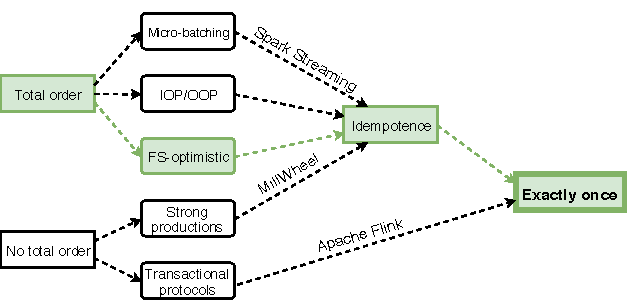
\includegraphics[width=0.47\textwidth]{pics/intro-approaches}
  \caption{The approaches for exactly-once processing}
  \label {approaches}
\end{figure}

In this work, we introduce the OOP-based architecture that allows us to leave only one buffer per computational pipeline while achieving determinism, and therefore, exactly-once. Our speculative approach is based on the special limited set of operations that are enough to express any stateful transformation and can be implemented in an optimistic manner. Such behavior is achieved using {\em drifting state} that allows a state to flow along a stream. In sections~\ref{fs-short-model} and~\ref{fs-short-discussion} we explain the main ideas behind our model. In~\ref{fs-short-experiments} we demonstrate that our approach can significantly outperform an industrial alternative within a real-life problem. 


\section {Problem statement}
\label {fs-short-model}

We found that only two operations are required to implement any stateful transformation:

\begin {description}
  \item [Map] applies a user-defined function to the payload of an input item and returns a sequence of data items with transformed payloads. 
  \item [Grouping] constructs a single item containing a set of consecutive items that have the same value of load-balancing function. The maximum number of items is defined by parameter $Window Size$. 
\end {description}

The stream processing is specified by a logical execution graph. Each vertex of the graph represents a single operation on data items, and edges describe the order between operations. Our model allows cycles in the graph while such graphs are commonly assumed to be acyclic (DAGs). As our reduced set of operations doesn't allows arbitrary stateful operations, cycles are used to implement common stateful transformations is a form of $(In, State) \rightarrow (Out, NewState)$.

Distributed environment consists of multiple workers. The whole logical graph is executed on each worker. Each worker is assigned with a hash range to define the data items, which would be processed on the worker. Edges of logical graph are marked with load-balancing function. It is applied to data items and depending on the result routes data items to the corresponding worker.

Date items consist of user-defined $Payload$, which is processed by business-logic, and $Meta$ which is handled with \FlameStream\ engine. $Meta$ is assigned to input events on system's entry. The main purpose of $Meta$ is to impose the total order on data items. All operations preserve this order. Any additional items produced by an operation are placed between the item being processed and the next item.


The output item of the grouping is assignd with the same $Meta$ as the last item in the output group. It is important to notice that grouping is the only operation that maintaines a state.

An important special case of grouping with $Window Size = 2$  provides for realization of stateful calculations with drifting state techniques.  

Indeed, consider a map operation that follows the grouping and sends its output to the grouping input. This map operation receives a pair of its previous output considered as the state object, and new incoming item from the source stream. The map operation calculates new state object and sends it back as the grouping input. 

{\bf Detail drifting state}

More details are provided in the optimistic aproach analysis paper~\cite{we2018seim}.


\section {Preliminary experiments}
\label {fs-short-experiments}

We conducted a series of experiments to estimate the performance of our prototype. We used a problem of building an incremental inverted index as a stream processing benchmark, because this task requires stateful operations and its computational flow contains network shuffle that can violate the ordering constraints enabling evaluation of our optimistic techniques. In the real-world, such scenario can be found in freshness-aware systems, e.g., news processing engines.

We used an industrial solution, Apache Flink, for the comparison. The computational pipeline is expressed as typical MapReduce-like transformation: map is used for splitting document into postings, and reduce - for grouping them by word and combining into the posting lists. We employ an optimistic approach to impose order before reduce stage, while in Apach Flink we set a buffer that were flushed on punctuations.

Our experiments were performed on the cluster of 10 Amazon EC2 micro instances with 1GB RAM and 1 core CPU with 10000 Wikipedia articles as a dataset.

Figure~\ref{performance} shows the latencies distributions of \FlameStream\ and Flink within distinct times between checkpoints and different consistency guarantees. The input rate is fixed at 50 documents per second.

At the initial point, \FlameStream\ provides the similar latencies for {\it at most once} semantics. However, for {\it exactly once semantics}, Flink's latency is dramatically higher and it directly depends on the time between checkpoints. Such behavior is expected, because unlike \FlameStream, Flink needs to take state snapshot and release output items within a single transaction in order to preserve exactly once semantics.

\begin{figure}[htbp]
  \centering
  \includegraphics[width=0.47\textwidth]{pics/comparison}
  \caption{The comparison in latencies between FlameStream and Flink for different consistency semantics}
  \label {performance}
\end{figure}


% \section {Related work}
% \label {fs-short-related}

\section {Conclusion}
\label {fs-short-conclusion}

We proposed a novel architecture based on speculative stateful model that allows to achieve exactly-once semantics with low overhead. Experiments demonstrated that our approach can significantly outperform an alternative solution under exactly-once requirement.

\bibliographystyle{ACM-Reference-Format}
\bibliography{../../bibliography/flame-stream}

\end {document}

\endinput
